\documentclass[conference]{IEEEtran}
\IEEEoverridecommandlockouts
\usepackage{cite}
\usepackage{amsmath,amssymb,amsfonts}
\usepackage{algorithmic}
\usepackage{graphicx}
\usepackage{textcomp}
\usepackage{xcolor}
\usepackage{listings}

\lstset{
    language=[LaTeX]TeX,
    basicstyle=\ttfamily\footnotesize,
    breaklines=true,
    breakatwhitespace=false,
    frame=single,
    numbers=none,
    showstringspaces=false,
    tabsize=2,
    backgroundcolor=\color{gray!5},
    rulecolor=\color{black!40},
    columns=flexible,
    keepspaces=true
}

\def\BibTeX{{\rm B\kern-.05em{\sc i\kern-.025em b}\kern-.08em
    T\kern-.1667em\lower.7ex\hbox{E}\kern-.125emX}}

\begin{document}

% ==================== COVER PAGE ====================
\begin{titlepage}
\centering
\vspace*{0.5cm}

{\bfseries\large Mata Kuliah Workshop Pemrograman Framework \par}
\vspace{0.3cm}
{\bfseries\Large LAPORAN E - GOVERNANCE \par}
\vspace{0.2cm}
{\bfseries\Large Sistem Pengajuan Subsidi Pupuk Kabupaten Mojokerto \par}

\vfill

\includegraphics[width=0.45\textwidth]{image1.png}
\vfill

{\normalsize
Dosen Pengampu: \par
\vspace{0.1cm}
Amma Liesvarastranta Haz, S.Tr.T., M.T. \par
\vspace{0.6cm}
Disusun Oleh: \par
\vspace{0.1cm}
Syarifatullah Ceva Efendy (312521002) \par
Selby Wafi Nurjuan (3125521018) \par
}

\vfill

{\bfseries\large PROGRAM STUDI D3 TEKNIK INFORMATIKA PSDKU LAMONGAN \par}
\vspace{0.1cm}
{\bfseries\large DEPARTEMEN TEKNIK INFORMATIKA DAN KOMPUTER \par}
\vspace{0.1cm}
{\bfseries\large POLITEKNIK ELEKTRONIKA NEGERI SURABAYA \par}
\vspace{0.1cm}
{\bfseries\large 2026 \par}
\vspace*{0.5cm}

\end{titlepage}
\clearpage

% ==================== BAB I ====================
\title{E-Pupuk: Sistem Pengajuan Subsidi Pupuk Kabupaten Mojokerto Berbasis Data Terbuka Pemerintah\\
\thanks{Laporan Progres Mata Kuliah Workshop Pemrograman Framework, D3 Teknik Informatika PSDKU Lamongan, PENS.}
}

\author{\IEEEauthorblockN{Syarifatullah Ceva Efendy\textsuperscript{1}, Selby Wafi Nurjuan\textsuperscript{2}}
\IEEEauthorblockA{\textit{D3 Teknik Informatika PSDKU Lamongan} \\
\textit{Departemen Teknik Informatika dan Komputer} \\
\textit{Politeknik Elektronika Negeri Surabaya (PENS)}\\
Lamongan, Indonesia \\
\textsuperscript{1}312521002@student.pens.ac.id, \textsuperscript{2}3125521018@student.pens.ac.id}
}

\maketitle

\begin{abstract}
Pengelolaan dan distribusi pupuk bersubsidi merupakan elemen vital dalam menjaga stabilitas produktivitas sektor pertanian di Kabupaten Mojokerto. Kendati demikian, mekanisme pengelolaan manual dan fragmentasi data alokasi sering memicu ketidakteraturan kuota, keterlambatan verifikasi pengajuan, serta potensi penyaluran yang tidak tepat sasaran. Penelitian ini mengusulkan pengembangan E-Pupuk, sistem informasi berbasis web terintegrasi yang memanfaatkan data terbuka pemerintah (\textit{Open Government Data}) alokasi Rencana Definitif Kebutuhan Kelompok (RDKK) secara dinamis. Kebaharuan (\textit{novelty}) dari sistem ini terletak pada penerapan validasi kuota otomatis berbasis aturan (\textit{rule-based quota checking}) yang diselaraskan dengan verifikasi geospasial batas lahan (\textit{geotagging}), alur verifikasi digital berjenjang (\textit{multi-tier verification}) antara Petani, Petugas Penyuluh Lapangan (PPL), dan Dinas Pertanian, serta penerbitan bukti tebus alokasi digital dengan \textit{dynamic QR code token} guna mengeliminasi risiko klaim ganda. Arsitektur sistem dibangun dengan model terpisah (\textit{decoupled}) menggunakan FastAPI (Python) pada sisi \textit{backend REST API}, PostgreSQL sebagai basis data relasional berkinerja tinggi, React.js dengan TypeScript pada sisi antarmuka \textit{frontend}, serta proteksi akses menggunakan \textit{Role-Based Access Control} (RBAC) berbasis JSON Web Token (JWT). Metode validasi sistem dilakukan secara menyeluruh melalui pengujian fungsionalitas menggunakan \textit{Black Box Testing} berbasis skenario peran ganda serta evaluasi penerimaan pengguna menggunakan metode \textit{System Usability Scale} (SUS) terhadap perwakilan kelompok tani dan petugas lapangan. Hasil pengujian menunjukkan persentase keberhasilan sistem mencapai XX,XX\% pada pengujian fungsionalitas \textit{Black Box Testing} dan skor usabilitas sebesar XX,XX\% pada evaluasi \textit{System Usability Scale} (SUS), yang membuktikan bahwa E-Pupuk berhasil mengotomatisasi validasi kuota, meningkatkan akurasi data pengajuan, serta menyediakan transparansi realisasi distribusi pupuk bersubsidi secara tepat waktu, efektif, dan akuntabel.
\end{abstract}

\begin{IEEEkeywords}
e-Governance, E-Pupuk, Subsidi Pupuk, Open Government Data, RDKK, FastAPI, React, Role-Based Access Control, QR Code, Black Box Testing, System Usability Scale.
\end{IEEEkeywords}

\section{Introduction}  
Perkembangan teknologi informasi dan komunikasi (TIK) mendorong transformasi tata kelola pemerintahan menuju \textit{e-Governance} yang transparan, partisipatif, efisien, dan akuntabel \cite{b1}. Salah satu pilar penting dalam modernisasi tata kelola sektor publik adalah pemanfaatan data terbuka pemerintah (\textit{Open Government Data}) sebagai instrumen transparansi dan akurasi pengambilan kebijakan publik \cite{b2}, \cite{b3}. Pemanfaatan data terbuka tidak hanya membuka akses informasi bagi publik, melainkan juga berperan sebagai fondasi integrasi layanan antarinstitusi guna mereduksi inefisiensi administratif \cite{b3}, khususnya dalam pengelolaan rantai pasok dan bantuan publik pada sektor agrikultur \cite{b6}.

Dalam konteks ketahanan pangan regional, Pemerintah Kabupaten Mojokerto secara periodik menyalurkan program pupuk bersubsidi guna membantu kelompok tani menekan ongkos produksi dan mempertahankan stabilitas hasil panen \cite{b5}. Alokasi volume pupuk subsidi ini mengacu pada dokumen Rencana Definitif Kebutuhan Kelompok (RDKK) yang disusun secara musyawarah oleh kelompok tani untuk kemudian divalidasi oleh instansi dinas teknis setempat \cite{b4}. Meskipun regulasi kuota telah diatur secara normatif, kenyataan operasional di tingkat lapangan kerap menemui kendala fragmentasi pendataan, keterlambatan pelaporan berkas fisik, tingginya potensi kekeliruan rekapitulasi data petani, serta kerentanan distorsi penyaluran alokasi kuota kepada pihak yang tidak memenuhi kualifikasi \cite{b5}, \cite{b7}.

Kondisi faktual tersebut semakin diperparah dengan ketiadaan saluran informasi digital interaktif bagi para petani, sehingga mereka mengalami kendala dalam memeriksa sisa hak kuota kelompok dan status pemrosesan berkas secara mandiri \cite{b7}. Di sisi lain, Petugas Penyuluh Lapangan (PPL) terbebani proses administrasi manual yang memakan waktu lama saat melakukan verifikasi fisik lahan dan keabsahan dokumen permohonan \cite{b6}. Dari perspektif regulator, pihak Dinas Pertanian menghadapi hambatan dalam melakukan pengawasan realisasi serapan pupuk secara seketika (\textit{real-time}), sehingga sulit mengidentifikasi anomali penyaluran sejak dini \cite{b3}, \cite{b5}.

Guna memecahkan kendala sistemik tersebut, penelitian ini mengembangkan \textbf{E-Pupuk: Sistem Pengajuan Subsidi Pupuk Kabupaten Mojokerto Berbasis Data Terbuka Pemerintah}. E-Pupuk dirancang sebagai platform web komprehensif yang mengintegrasikan pendataan spasial petani dan poligon lahan, sinkronisasi kuota berbasis dataset terbuka RDKK, alur persetujuan verifikasi digital berjenjang, penerbitan tanda bukti tebus alokasi terenkripsi kode batang respons cepat (\textit{QR Code}), serta dasbor analitik distribusi eksekutif terpusat bagi jajaran dinas terkait \cite{b6}, \cite{b7}.

\section{Tinjauan Pustaka}
\subsection{E-Governance dan Ekosistem Open Government Data}
Implementasi teknologi informasi pada sektor pemerintahan atau \textit{e-Governance} secara fundamental bertujuan mentransformasi interaksi antara pemerintah, masyarakat, dan pelaku usaha ke arah yang lebih transparan dan akuntabel \cite{b1}. Janssen dkk. menekankan bahwa pemanfaatan data terbuka pemerintah (\textit{Open Government Data}) membuka peluang besar untuk meruntuhkan silo birokrasi, memberdayakan masyarakat, dan menstimulasi efisiensi operasional layanan publik berbasis data valid \cite{b2}. Kajian komprehensif oleh Attard dkk. menegaskan bahwa keberhasilan inisiatif data terbuka sangat bergantung pada ketersediaan data yang terstruktur, mudah diakses, serta dapat digunakan secara langsung oleh aplikasi pihak ketiga maupun sistem informasi publik \cite{b3}. Dalam domain pertanian di Indonesia, Ahmad menguraikan bahwa transparansi data alokasi pupuk bersubsidi melalui portal data terbuka dapat menekan potensi kecurangan dan memastikan asas keadilan bagi petani penggarap \cite{b6}. Pada arsitektur E-Pupuk, dataset terbuka pemerintah daerah digunakan sebagai titik acuan data awal (\textit{data-seeding}) untuk memvalidasi batas atas kuota per kelompok tani secara transparan.

\subsection{Regulasi RDKK dan Dinamika Distribusi Pupuk Subsidi}
Rencana Definitif Kebutuhan Kelompok (RDKK) secara elektronik atau e-RDKK merupakan instrumen regulasi utama yang ditetapkan Kementerian Pertanian Republik Indonesia untuk merencanakan alokasi pupuk bersubsidi secara berjenjang mulai dari tingkat desa hingga nasional \cite{b4}. Kendati kerangka elektronik e-RDKK telah digulirkan secara terpusat, laporan evaluasi Dinas Pertanian Kabupaten Mojokerto menggarisbawahi bahwa pada tingkat implementasi operasional kecamatan masih terdapat celah koordinasi, keterlambatan pemutakhiran data kepemilikan lahan, serta kendala validasi fisik di lapangan oleh petugas penyuluh \cite{b5}. Penelitian Suryanto dkk. membuktikan bahwa integrasi data alokasi pupuk dengan pemetaan geografis berbasis web secara signifikan mampu menyederhanakan pemantauan kuota dan mencegah tumpang-tindih permohonan antar-kelompok \cite{b7}. E-Pupuk menyempurnakan pendekatan ini dengan menghubungkan kuota RDKK terhadap validasi batas luas lahan secara langsung pada saat pengajuan diajukan oleh petani.

\subsection{Arsitektur Perangkat Lunak Web RESTful dan Asynchronous API}
Pengembangan aplikasi layanan publik modern mensyaratkan arsitektur yang tangguh, responsif, dan mudah dipelihara. Pola arsitektur terpisah (\textit{decoupled architecture}) memisahkan antarmuka pengguna (\textit{frontend}) dan penyedia layanan data (\textit{backend}) melalui antarmuka pertukaran data standar RESTful API \cite{b8}, \cite{b9}. Framework FastAPI dipilih dalam riset ini karena kemampuannya mengeksekusi komputasi konkurensi asinkron (\textit{asynchronous I/O}) berbasis standar ASGI Python, menyajikan performa latensi sangat rendah, serta menyediakan validasi tipe data otomatis melalui skema Pydantic \cite{b8}. Pada sisi antarmuka, library React.js yang dipadukan dengan bahasa TypeScript memberikan keandalan dalam merender antarmuka pengguna berbasis komponen reaktif secara cepat, menjamin kerapian kode skala besar, serta memfasilitasi interaksi pengguna yang adaptif terhadap perangkat seluler maupun desktop \cite{b9}, \cite{b15}.

\subsection{Keamanan Sistem dan Role-Based Access Control (RBAC)}
Sistem informasi tata kelola pemerintahan yang melibatkan berbagai entitas pengguna wajib mengimplementasikan kontrol otorisasi yang ketat. Standar keamanan National Institute of Standards and Technology (NIST) mendefinisikan \textit{Role-Based Access Control} (RBAC) sebagai metodologi penetapan izin akses berdasarkan peran fungsional pengguna dalam suatu organisasi \cite{b10}. Dalam E-Pupuk, RBAC diimplementasikan secara granular untuk membedakan hak akses antara Petani, Petugas Penyuluh Lapangan (PPL), Admin Kecamatan, dan Kepala Dinas Pertanian. Untuk menjamin komunikasi data yang nir-status (\textit{stateless}), sistem menerapkan standar tokenisasi \textit{JSON Web Token} (JWT) dengan enkripsi berbasis algoritma SHA-256 yang dikombinasikan dengan teknik \textit{hashing} kata sandi menggunakan pustaka Bcrypt, sehingga privasi dan integritas data pengguna terlindungi dari ancaman penyusupan tidak sah \cite{b11}.

\subsection{Verifikasi Geospasial dan Validasi Transaksi QR Code}
Validasi faktual keberadaan lahan pertanian menjadi faktor penentu dalam mencegah penyalahgunaan subsidi pupuk. Pemanfaatan koordinat geospasial (\textit{geotagging}) pada peta digital interaktif memungkinkan petugas PPL memverifikasi lokasi fisik lahan yang didaftarkan petani secara objektif \cite{b7}. Selain itu, teknologi kode respons cepat (\textit{QR Code}) terbukti efektif sebagai media verifikasi fisik yang cepat, murah, dan akurat dalam rantai pelacakan logistik maupun bukti transaksi resmi \cite{b12}. E-Pupuk mengimplementasikan generasi QR Code yang memuat tanda tangan kriptografis unik pada setiap lembar bukti alokasi yang telah disetujui, sehingga pihak kios penyalur dapat melakukan validasi keaslian dokumen secara instan dan mencegah penebusan berulang atas kuota yang sama \cite{b12}.

\subsection{Metodologi Pengujian dan Evaluasi Usabilitas Sistem}
Untuk menjamin kualitas dan keandalan sistem sebelum diterapkan secara luas, diperlukan metodologi rekayasa perangkat lunak yang sistematis. Pressman dan Maxim menjelaskan bahwa metode pengujian kotak hitam (\textit{Black Box Testing}) merupakan pendekatan esensial untuk memverifikasi fungsionalitas antarmuka dan keluaran sistem berdasarkan spesifikasi kebutuhan tanpa harus menganalisis kode internal secara langsung \cite{b13}. Di samping pengujian fungsional, penerimaan sistem oleh pengguna akhir dievaluasi menggunakan instrumen \textit{System Usability Scale} (SUS) yang dikembangkan oleh Brooke \cite{b14}. Instrumen SUS telah terbukti secara empiris sebagai alat ukur usabilitas standar industri dengan keandalan tinggi untuk menilai kemudahan belajar, efisiensi interaksi, dan tingkat kepuasan pengguna \cite{b14}, \cite{b16}. Prinsip-prinsip desain antarmuka responsif yang ramah pengguna juga diterapkan sesuai panduan Nielsen untuk memastikan petani dengan variasi literasi digital dapat mengoperasikan sistem tanpa kendala berarti \cite{b15}.

\subsection{Posisi dan Kebaharuan Sistem E-Pupuk}
Berdasarkan sintesis terhadap berbagai studi terdahulu, sistem E-Pupuk menempati posisi strategis yang menjembatani kesenjangan antara ketersediaan data terbuka pemerintah dengan otomatisasi alur kerja verifikasi lapangan di sektor pertanian. Perbandingan terhadap sistem konvensional menunjukkan bahwa E-Pupuk tidak sekadar mendigitalkan formulir pengajuan, melainkan menghadirkan kebaharuan integrasi validasi kuota otomatis terhubung dataset e-RDKK, pengecekan spasial lahan, pelacakan status berjenjang terverifikasi PPL, hingga penerbitan token tebus QR Code anti-pemalsuan. Integrasi menyeluruh ini menghadirkan ekosistem tata kelola distribusi pupuk bersubsidi Kabupaten Mojokerto yang akuntabel, transparan, dan terukur.

\begin{thebibliography}{00}
\bibitem{b1} R. Heeks, \textit{Implementing and Managing e-Government: An International Text}. London: SAGE Publications, 2006.
\bibitem{b2} M. Janssen, Y. Charalabidis, and A. Zuiderwijk, `Benefits, adoption barriers and myths of open data and open government,'' \textit{Information Systems Management}, vol. 29, no. 4, pp. 258--268, 2012.
\bibitem{b3} J. Attard, F. Orlandi, S. Scerri, and S. Auer, `A systematic review of open government data initiatives,'' \textit{Government Information Quarterly}, vol. 32, no. 4, pp. 399--418, 2015.
\bibitem{b4} Kementerian Pertanian Republik Indonesia, `Pedoman Pengelolaan Sistem Elektronik Rencana Definitif Kebutuhan Kelompok (e-RDKK),'' Kementerian Pertanian RI, Jakarta, 2021.
\bibitem{b5} Dinas Pertanian Kabupaten Mojokerto, `Laporan Evaluasi Penyaluran Pupuk Bersubsidi Kabupaten Mojokerto,'' Dinas Pertanian Kab. Mojokerto, Mojokerto, 2024.
\bibitem{b6} A. S. Ahmad, `Pemanfaatan Open Government Data untuk Transparansi Layanan Publik di Sektor Pertanian,'' \textit{Jurnal Teknologi dan Governance}, vol. 8, no. 1, pp. 45--56, 2023.
\bibitem{b7} R. Suryanto, H. Wibowo, dan M. Firdaus, `Rancang Bangun Sistem Informasi Distribusi Pupuk Bersubsidi Berbasis Web dan Geospasial,'' \textit{Jurnal RESTI (Rekayasa Sistem dan Teknologi Informasi)}, vol. 6, no. 3, pp. 412--419, 2022.
\bibitem{b8} M. S. L. Tiangolo, `FastAPI: Modern, High-Performance Web Framework for Python,'' 2023. [Online]. Available: https://fastapi.tiangolo.com/
\bibitem{b9} A. Freeman, \textit{Pro React 18: Intensive Modern Web Development}. New York: Apress, 2023.
\bibitem{b10} D. F. Ferraiolo, R. Sandhu, S. Gavrila, D. R. Kuhn, and R. Chandramouli, `Proposed NIST Standard for Role-Based Access Control,'' \textit{ACM Transactions on Information and System Security}, vol. 4, no. 3, pp. 224--274, 2001.
\bibitem{b11} M. B. Jones, J. Bradley, and N. Sakimura, `JSON Web Token (JWT),'' \textit{RFC 7519, Internet Engineering Task Force (IETF)}, 2015.
\bibitem{b12} T. Gao, D. Liu, and Y. Zhang, `Application of QR Code Technology in Traceability and Verification Systems,'' \textit{IEEE Access}, vol. 8, pp. 128450--128461, 2020.
\bibitem{b13} R. S. Pressman and B. R. Maxim, \textit{Software Engineering: A Practitioner's Approach}, 9th ed. New York: McGraw-Hill Education, 2020.
\bibitem{b14} J. Brooke, `SUS: A 'Quick and Dirty' Usability Scale,'' in \textit{Usability Evaluation in Industry}, P. W. Jordan, B. Thomas, I. L. McClelland, and B. Weerdmeester, Eds. London: Taylor \& Francis, 1996, pp. 189--194.
\bibitem{b15} J. Nielsen and R. Budiu, \textit{Mobile Usability: Usability Engineering in the Era of Responsive Design}. Berkeley: New Riders, 2013.
\bibitem{b16} D. Pramudita dan M. Muslikh, `Analisis Penerimaan Sistem Informasi Pertanian Digital Menggunakan Model Evaluasi Usabilitas,'' \textit{Jurnal Sistem Cerdas}, vol. 5, no. 2, pp. 98--109, 2022.
\end{thebibliography}

% ==================== PERALIHAN KE 1 KOLOM & LEMBAR BARU ====================
\clearpage
\onecolumn

% ==================== BAB II ====================
\section{Sumber Kode}
\label{sec:sumber_kode}

\begin{lstlisting}
\documentclass[conference]{IEEEtran}
\IEEEoverridecommandlockouts
\usepackage{cite}
\usepackage{amsmath,amssymb,amsfonts}
\usepackage{algorithmic}
\usepackage{graphicx}
\usepackage{textcomp}
\usepackage{xcolor}
\usepackage{listings}

\lstset{
    language=[LaTeX]TeX,
    basicstyle=\ttfamily\footnotesize,
    breaklines=true,
    breakatwhitespace=false,
    frame=single,
    numbers=none,
    showstringspaces=false,
    tabsize=2,
    backgroundcolor=\color{gray!5},
    rulecolor=\color{black!40},
    columns=flexible,
    keepspaces=true
}

\def\BibTeX{{\rm B\kern-.05em{\sc i\kern-.025em b}\kern-.08em
    T\kern-.1667em\lower.7ex\hbox{E}\kern-.125emX}}

\begin{document}

% ==================== COVER PAGE ====================
\begin{titlepage}
\centering
\vspace*{0.5cm}

{\bfseries\large Mata Kuliah Workshop Pemrograman Framework \par}
\vspace{0.3cm}
{\bfseries\Large LAPORAN E - GOVERNANCE \par}
\vspace{0.2cm}
{\bfseries\Large Sistem Pengajuan Subsidi Pupuk Kabupaten Mojokerto \par}

\vfill

\includegraphics[width=0.45\textwidth]{image1.png}
\vfill

{\normalsize
Dosen Pengampu: \par
\vspace{0.1cm}
Amma Liesvarastranta Haz, S.Tr.T., M.T. \par
\vspace{0.6cm}
Disusun Oleh: \par
\vspace{0.1cm}
Syarifatullah Ceva Efendy (312521002) \par
Selby Wafi Nurjuan (3125521018) \par
}

\vfill

{\bfseries\large PROGRAM STUDI D3 TEKNIK INFORMATIKA PSDKU LAMONGAN \par}
\vspace{0.1cm}
{\bfseries\large DEPARTEMEN TEKNIK INFORMATIKA DAN KOMPUTER \par}
\vspace{0.1cm}
{\bfseries\large POLITEKNIK ELEKTRONIKA NEGERI SURABAYA \par}
\vspace{0.1cm}
{\bfseries\large 2026 \par}
\vspace*{0.5cm}

\end{titlepage}
\clearpage

% ==================== BAB I ====================
\title{E-Pupuk: Sistem Pengajuan Subsidi Pupuk Kabupaten Mojokerto Berbasis Data Terbuka Pemerintah\\
\thanks{Laporan Progres Mata Kuliah Workshop Pemrograman Framework, D3 Teknik Informatika PSDKU Lamongan, PENS.}
}

\author{\IEEEauthorblockN{Syarifatullah Ceva Efendy\textsuperscript{1}, Selby Wafi Nurjuan\textsuperscript{2}}
\IEEEauthorblockA{\textit{D3 Teknik Informatika PSDKU Lamongan} \\
\textit{Departemen Teknik Informatika dan Komputer} \\
\textit{Politeknik Elektronika Negeri Surabaya (PENS)}\\
Lamongan, Indonesia \\
\textsuperscript{1}312521002@student.pens.ac.id, \textsuperscript{2}3125521018@student.pens.ac.id}
}

\maketitle

\begin{abstract}
Pengelolaan dan distribusi pupuk bersubsidi merupakan elemen vital dalam menjaga stabilitas produktivitas sektor pertanian di Kabupaten Mojokerto. Kendati demikian, mekanisme pengelolaan manual dan fragmentasi data alokasi sering memicu ketidakteraturan kuota, keterlambatan verifikasi pengajuan, serta potensi penyaluran yang tidak tepat sasaran. Penelitian ini mengusulkan pengembangan E-Pupuk, sistem informasi berbasis web terintegrasi yang memanfaatkan data terbuka pemerintah (\textit{Open Government Data}) alokasi Rencana Definitif Kebutuhan Kelompok (RDKK) secara dinamis. Kebaharuan (\textit{novelty}) dari sistem ini terletak pada penerapan validasi kuota otomatis berbasis aturan (\textit{rule-based quota checking}) yang diselaraskan dengan verifikasi geospasial batas lahan (\textit{geotagging}), alur verifikasi digital berjenjang (\textit{multi-tier verification}) antara Petani, Petugas Penyuluh Lapangan (PPL), dan Dinas Pertanian, serta penerbitan bukti tebus alokasi digital dengan \textit{dynamic QR code token} guna mengeliminasi risiko klaim ganda. Arsitektur sistem dibangun dengan model terpisah (\textit{decoupled}) menggunakan FastAPI (Python) pada sisi \textit{backend REST API}, PostgreSQL sebagai basis data relasional berkinerja tinggi, React.js dengan TypeScript pada sisi antarmuka \textit{frontend}, serta proteksi akses menggunakan \textit{Role-Based Access Control} (RBAC) berbasis JSON Web Token (JWT). Metode validasi sistem dilakukan secara menyeluruh melalui pengujian fungsionalitas menggunakan \textit{Black Box Testing} berbasis skenario peran ganda serta evaluasi penerimaan pengguna menggunakan metode \textit{System Usability Scale} (SUS) terhadap perwakilan kelompok tani dan petugas lapangan. Hasil pengujian menunjukkan persentase keberhasilan sistem mencapai XX,XX\% pada pengujian fungsionalitas \textit{Black Box Testing} dan skor usabilitas sebesar XX,XX\% pada evaluasi \textit{System Usability Scale} (SUS), yang membuktikan bahwa E-Pupuk berhasil mengotomatisasi validasi kuota, meningkatkan akurasi data pengajuan, serta menyediakan transparansi realisasi distribusi pupuk bersubsidi secara tepat waktu, efektif, dan akuntabel.
\end{abstract}

\begin{IEEEkeywords}
e-Governance, E-Pupuk, Subsidi Pupuk, Open Government Data, RDKK, FastAPI, React, Role-Based Access Control, QR Code, Black Box Testing, System Usability Scale.
\end{IEEEkeywords}

\section{Introduction}  
Perkembangan teknologi informasi dan komunikasi (TIK) mendorong transformasi tata kelola pemerintahan menuju \textit{e-Governance} yang transparan, partisipatif, efisien, dan akuntabel \cite{b1}. Salah satu pilar penting dalam modernisasi tata kelola sektor publik adalah pemanfaatan data terbuka pemerintah (\textit{Open Government Data}) sebagai instrumen transparansi dan akurasi pengambilan kebijakan publik \cite{b2}, \cite{b3}. Pemanfaatan data terbuka tidak hanya membuka akses informasi bagi publik, melainkan juga berperan sebagai fondasi integrasi layanan antarinstitusi guna mereduksi inefisiensi administratif \cite{b3}, khususnya dalam pengelolaan rantai pasok dan bantuan publik pada sektor agrikultur \cite{b6}.

Dalam konteks ketahanan pangan regional, Pemerintah Kabupaten Mojokerto secara periodik menyalurkan program pupuk bersubsidi guna membantu kelompok tani menekan ongkos produksi dan mempertahankan stabilitas hasil panen \cite{b5}. Alokasi volume pupuk subsidi ini mengacu pada dokumen Rencana Definitif Kebutuhan Kelompok (RDKK) yang disusun secara musyawarah oleh kelompok tani untuk kemudian divalidasi oleh instansi dinas teknis setempat \cite{b4}. Meskipun regulasi kuota telah diatur secara normatif, kenyataan operasional di tingkat lapangan kerap menemui kendala fragmentasi pendataan, keterlambatan pelaporan berkas fisik, tingginya potensi kekeliruan rekapitulasi data petani, serta kerentanan distorsi penyaluran alokasi kuota kepada pihak yang tidak memenuhi kualifikasi \cite{b5}, \cite{b7}.

Kondisi faktual tersebut semakin diperparah dengan ketiadaan saluran informasi digital interaktif bagi para petani, sehingga mereka mengalami kendala dalam memeriksa sisa hak kuota kelompok dan status pemrosesan berkas secara mandiri \cite{b7}. Di sisi lain, Petugas Penyuluh Lapangan (PPL) terbebani proses administrasi manual yang memakan waktu lama saat melakukan verifikasi fisik lahan dan keabsahan dokumen permohonan \cite{b6}. Dari perspektif regulator, pihak Dinas Pertanian menghadapi hambatan dalam melakukan pengawasan realisasi serapan pupuk secara seketika (\textit{real-time}), sehingga sulit mengidentifikasi anomali penyaluran sejak dini \cite{b3}, \cite{b5}.

Guna memecahkan kendala sistemik tersebut, penelitian ini mengembangkan \textbf{E-Pupuk: Sistem Pengajuan Subsidi Pupuk Kabupaten Mojokerto Berbasis Data Terbuka Pemerintah}. E-Pupuk dirancang sebagai platform web komprehensif yang mengintegrasikan pendataan spasial petani dan poligon lahan, sinkronisasi kuota berbasis dataset terbuka RDKK, alur persetujuan verifikasi digital berjenjang, penerbitan tanda bukti tebus alokasi terenkripsi kode batang respons cepat (\textit{QR Code}), serta dasbor analitik distribusi eksekutif terpusat bagi jajaran dinas terkait \cite{b6}, \cite{b7}.

\section{Tinjauan Pustaka}
\subsection{E-Governance dan Ekosistem Open Government Data}
Implementasi teknologi informasi pada sektor pemerintahan atau \textit{e-Governance} secara fundamental bertujuan mentransformasi interaksi antara pemerintah, masyarakat, dan pelaku usaha ke arah yang lebih transparan dan akuntabel \cite{b1}. Janssen dkk. menekankan bahwa pemanfaatan data terbuka pemerintah (\textit{Open Government Data}) membuka peluang besar untuk meruntuhkan silo birokrasi, memberdayakan masyarakat, dan menstimulasi efisiensi operasional layanan publik berbasis data valid \cite{b2}. Kajian komprehensif oleh Attard dkk. menegaskan bahwa keberhasilan inisiatif data terbuka sangat bergantung pada ketersediaan data yang terstruktur, mudah diakses, serta dapat digunakan secara langsung oleh aplikasi pihak ketiga maupun sistem informasi publik \cite{b3}. Dalam domain pertanian di Indonesia, Ahmad menguraikan bahwa transparansi data alokasi pupuk bersubsidi melalui portal data terbuka dapat menekan potensi kecurangan dan memastikan asas keadilan bagi petani penggarap \cite{b6}. Pada arsitektur E-Pupuk, dataset terbuka pemerintah daerah digunakan sebagai titik acuan data awal (\textit{data-seeding}) untuk memvalidasi batas atas kuota per kelompok tani secara transparan.

\subsection{Regulasi RDKK dan Dinamika Distribusi Pupuk Subsidi}
Rencana Definitif Kebutuhan Kelompok (RDKK) secara elektronik atau e-RDKK merupakan instrumen regulasi utama yang ditetapkan Kementerian Pertanian Republik Indonesia untuk merencanakan alokasi pupuk bersubsidi secara berjenjang mulai dari tingkat desa hingga nasional \cite{b4}. Kendati kerangka elektronik e-RDKK telah digulirkan secara terpusat, laporan evaluasi Dinas Pertanian Kabupaten Mojokerto menggarisbawahi bahwa pada tingkat implementasi operasional kecamatan masih terdapat celah koordinasi, keterlambatan pemutakhiran data kepemilikan lahan, serta kendala validasi fisik di lapangan oleh petugas penyuluh \cite{b5}. Penelitian Suryanto dkk. membuktikan bahwa integrasi data alokasi pupuk dengan pemetaan geografis berbasis web secara signifikan mampu menyederhanakan pemantauan kuota dan mencegah tumpang-tindih permohonan antar-kelompok \cite{b7}. E-Pupuk menyempurnakan pendekatan ini dengan menghubungkan kuota RDKK terhadap validasi batas luas lahan secara langsung pada saat pengajuan diajukan oleh petani.

\subsection{Arsitektur Perangkat Lunak Web RESTful dan Asynchronous API}
Pengembangan aplikasi layanan publik modern mensyaratkan arsitektur yang tangguh, responsif, dan mudah dipelihara. Pola arsitektur terpisah (\textit{decoupled architecture}) memisahkan antarmuka pengguna (\textit{frontend}) dan penyedia layanan data (\textit{backend}) melalui antarmuka pertukaran data standar RESTful API \cite{b8}, \cite{b9}. Framework FastAPI dipilih dalam riset ini karena kemampuannya mengeksekusi komputasi konkurensi asinkron (\textit{asynchronous I/O}) berbasis standar ASGI Python, menyajikan performa latensi sangat rendah, serta menyediakan validasi tipe data otomatis melalui skema Pydantic \cite{b8}. Pada sisi antarmuka, library React.js yang dipadukan dengan bahasa TypeScript memberikan keandalan dalam merender antarmuka pengguna berbasis komponen reaktif secara cepat, menjamin kerapian kode skala besar, serta memfasilitasi interaksi pengguna yang adaptif terhadap perangkat seluler maupun desktop \cite{b9}, \cite{b15}.

\subsection{Keamanan Sistem dan Role-Based Access Control (RBAC)}
Sistem informasi tata kelola pemerintahan yang melibatkan berbagai entitas pengguna wajib mengimplementasikan kontrol otorisasi yang ketat. Standar keamanan National Institute of Standards and Technology (NIST) mendefinisikan \textit{Role-Based Access Control} (RBAC) sebagai metodologi penetapan izin akses berdasarkan peran fungsional pengguna dalam suatu organisasi \cite{b10}. Dalam E-Pupuk, RBAC diimplementasikan secara granular untuk membedakan hak akses antara Petani, Petugas Penyuluh Lapangan (PPL), Admin Kecamatan, dan Kepala Dinas Pertanian. Untuk menjamin komunikasi data yang nir-status (\textit{stateless}), sistem menerapkan standar tokenisasi \textit{JSON Web Token} (JWT) dengan enkripsi berbasis algoritma SHA-256 yang dikombinasikan dengan teknik \textit{hashing} kata sandi menggunakan pustaka Bcrypt, sehingga privasi dan integritas data pengguna terlindungi dari ancaman penyusupan tidak sah \cite{b11}.

\subsection{Verifikasi Geospasial dan Validasi Transaksi QR Code}
Validasi faktual keberadaan lahan pertanian menjadi faktor penentu dalam mencegah penyalahgunaan subsidi pupuk. Pemanfaatan koordinat geospasial (\textit{geotagging}) pada peta digital interaktif memungkinkan petugas PPL memverifikasi lokasi fisik lahan yang didaftarkan petani secara objektif \cite{b7}. Selain itu, teknologi kode respons cepat (\textit{QR Code}) terbukti efektif sebagai media verifikasi fisik yang cepat, murah, dan akurat dalam rantai pelacakan logistik maupun bukti transaksi resmi \cite{b12}. E-Pupuk mengimplementasikan generasi QR Code yang memuat tanda tangan kriptografis unik pada setiap lembar bukti alokasi yang telah disetujui, sehingga pihak kios penyalur dapat melakukan validasi keaslian dokumen secara instan dan mencegah penebusan berulang atas kuota yang sama \cite{b12}.

\subsection{Metodologi Pengujian dan Evaluasi Usabilitas Sistem}
Untuk menjamin kualitas dan keandalan sistem sebelum diterapkan secara luas, diperlukan metodologi rekayasa perangkat lunak yang sistematis. Pressman dan Maxim menjelaskan bahwa metode pengujian kotak hitam (\textit{Black Box Testing}) merupakan pendekatan esensial untuk memverifikasi fungsionalitas antarmuka dan keluaran sistem berdasarkan spesifikasi kebutuhan tanpa harus menganalisis kode internal secara langsung \cite{b13}. Di samping pengujian fungsional, penerimaan sistem oleh pengguna akhir dievaluasi menggunakan instrumen \textit{System Usability Scale} (SUS) yang dikembangkan oleh Brooke \cite{b14}. Instrumen SUS telah terbukti secara empiris sebagai alat ukur usabilitas standar industri dengan keandalan tinggi untuk menilai kemudahan belajar, efisiensi interaksi, dan tingkat kepuasan pengguna \cite{b14}, \cite{b16}. Prinsip-prinsip desain antarmuka responsif yang ramah pengguna juga diterapkan sesuai panduan Nielsen untuk memastikan petani dengan variasi literasi digital dapat mengoperasikan sistem tanpa kendala berarti \cite{b15}.

\subsection{Posisi dan Kebaharuan Sistem E-Pupuk}
Berdasarkan sintesis terhadap berbagai studi terdahulu, sistem E-Pupuk menempati posisi strategis yang menjembatani kesenjangan antara ketersediaan data terbuka pemerintah dengan otomatisasi alur kerja verifikasi lapangan di sektor pertanian. Perbandingan terhadap sistem konvensional menunjukkan bahwa E-Pupuk tidak sekadar mendigitalkan formulir pengajuan, melainkan menghadirkan kebaharuan integrasi validasi kuota otomatis terhubung dataset e-RDKK, pengecekan spasial lahan, pelacakan status berjenjang terverifikasi PPL, hingga penerbitan token tebus QR Code anti-pemalsuan. Integrasi menyeluruh ini menghadirkan ekosistem tata kelola distribusi pupuk bersubsidi Kabupaten Mojokerto yang akuntabel, transparan, dan terukur.

\begin{thebibliography}{00}
\bibitem{b1} R. Heeks, \textit{Implementing and Managing e-Government: An International Text}. London: SAGE Publications, 2006.
\bibitem{b2} M. Janssen, Y. Charalabidis, and A. Zuiderwijk, `Benefits, adoption barriers and myths of open data and open government,'' \textit{Information Systems Management}, vol. 29, no. 4, pp. 258--268, 2012.
\bibitem{b3} J. Attard, F. Orlandi, S. Scerri, and S. Auer, `A systematic review of open government data initiatives,'' \textit{Government Information Quarterly}, vol. 32, no. 4, pp. 399--418, 2015.
\bibitem{b4} Kementerian Pertanian Republik Indonesia, `Pedoman Pengelolaan Sistem Elektronik Rencana Definitif Kebutuhan Kelompok (e-RDKK),'' Kementerian Pertanian RI, Jakarta, 2021.
\bibitem{b5} Dinas Pertanian Kabupaten Mojokerto, `Laporan Evaluasi Penyaluran Pupuk Bersubsidi Kabupaten Mojokerto,'' Dinas Pertanian Kab. Mojokerto, Mojokerto, 2024.
\bibitem{b6} A. S. Ahmad, `Pemanfaatan Open Government Data untuk Transparansi Layanan Publik di Sektor Pertanian,'' \textit{Jurnal Teknologi dan Governance}, vol. 8, no. 1, pp. 45--56, 2023.
\bibitem{b7} R. Suryanto, H. Wibowo, dan M. Firdaus, `Rancang Bangun Sistem Informasi Distribusi Pupuk Bersubsidi Berbasis Web dan Geospasial,'' \textit{Jurnal RESTI (Rekayasa Sistem dan Teknologi Informasi)}, vol. 6, no. 3, pp. 412--419, 2022.
\bibitem{b8} M. S. L. Tiangolo, `FastAPI: Modern, High-Performance Web Framework for Python,'' 2023. [Online]. Available: https://fastapi.tiangolo.com/
\bibitem{b9} A. Freeman, \textit{Pro React 18: Intensive Modern Web Development}. New York: Apress, 2023.
\bibitem{b10} D. F. Ferraiolo, R. Sandhu, S. Gavrila, D. R. Kuhn, and R. Chandramouli, `Proposed NIST Standard for Role-Based Access Control,'' \textit{ACM Transactions on Information and System Security}, vol. 4, no. 3, pp. 224--274, 2001.
\bibitem{b11} M. B. Jones, J. Bradley, and N. Sakimura, `JSON Web Token (JWT),'' \textit{RFC 7519, Internet Engineering Task Force (IETF)}, 2015.
\bibitem{b12} T. Gao, D. Liu, and Y. Zhang, `Application of QR Code Technology in Traceability and Verification Systems,'' \textit{IEEE Access}, vol. 8, pp. 128450--128461, 2020.
\bibitem{b13} R. S. Pressman and B. R. Maxim, \textit{Software Engineering: A Practitioner's Approach}, 9th ed. New York: McGraw-Hill Education, 2020.
\bibitem{b14} J. Brooke, `SUS: A 'Quick and Dirty' Usability Scale,'' in \textit{Usability Evaluation in Industry}, P. W. Jordan, B. Thomas, I. L. McClelland, and B. Weerdmeester, Eds. London: Taylor \& Francis, 1996, pp. 189--194.
\bibitem{b15} J. Nielsen and R. Budiu, \textit{Mobile Usability: Usability Engineering in the Era of Responsive Design}. Berkeley: New Riders, 2013.
\bibitem{b16} D. Pramudita dan M. Muslikh, `Analisis Penerimaan Sistem Informasi Pertanian Digital Menggunakan Model Evaluasi Usabilitas,'' \textit{Jurnal Sistem Cerdas}, vol. 5, no. 2, pp. 98--109, 2022.
\end{thebibliography}

% ==================== PERALIHAN KE 1 KOLOM & LEMBAR BARU ====================
\clearpage
\onecolumn

% ==================== BAB II ====================
\section{Sumber Kode}
\label{sec:sumber_kode}

\clearpage

% ==================== BAB III ====================
\section{Design System}
\label{sec:design_system}

Design system E-Pupuk merancang visual konsisten, komponen antarmuka modular, skema warna yang harmonis, dan elemen navigasi intuitif untuk pengguna dari berbagai peran (Petani, PPL, Admin, dan Pimpinan Dinas).

\begin{figure}[htbp]
    \centering
    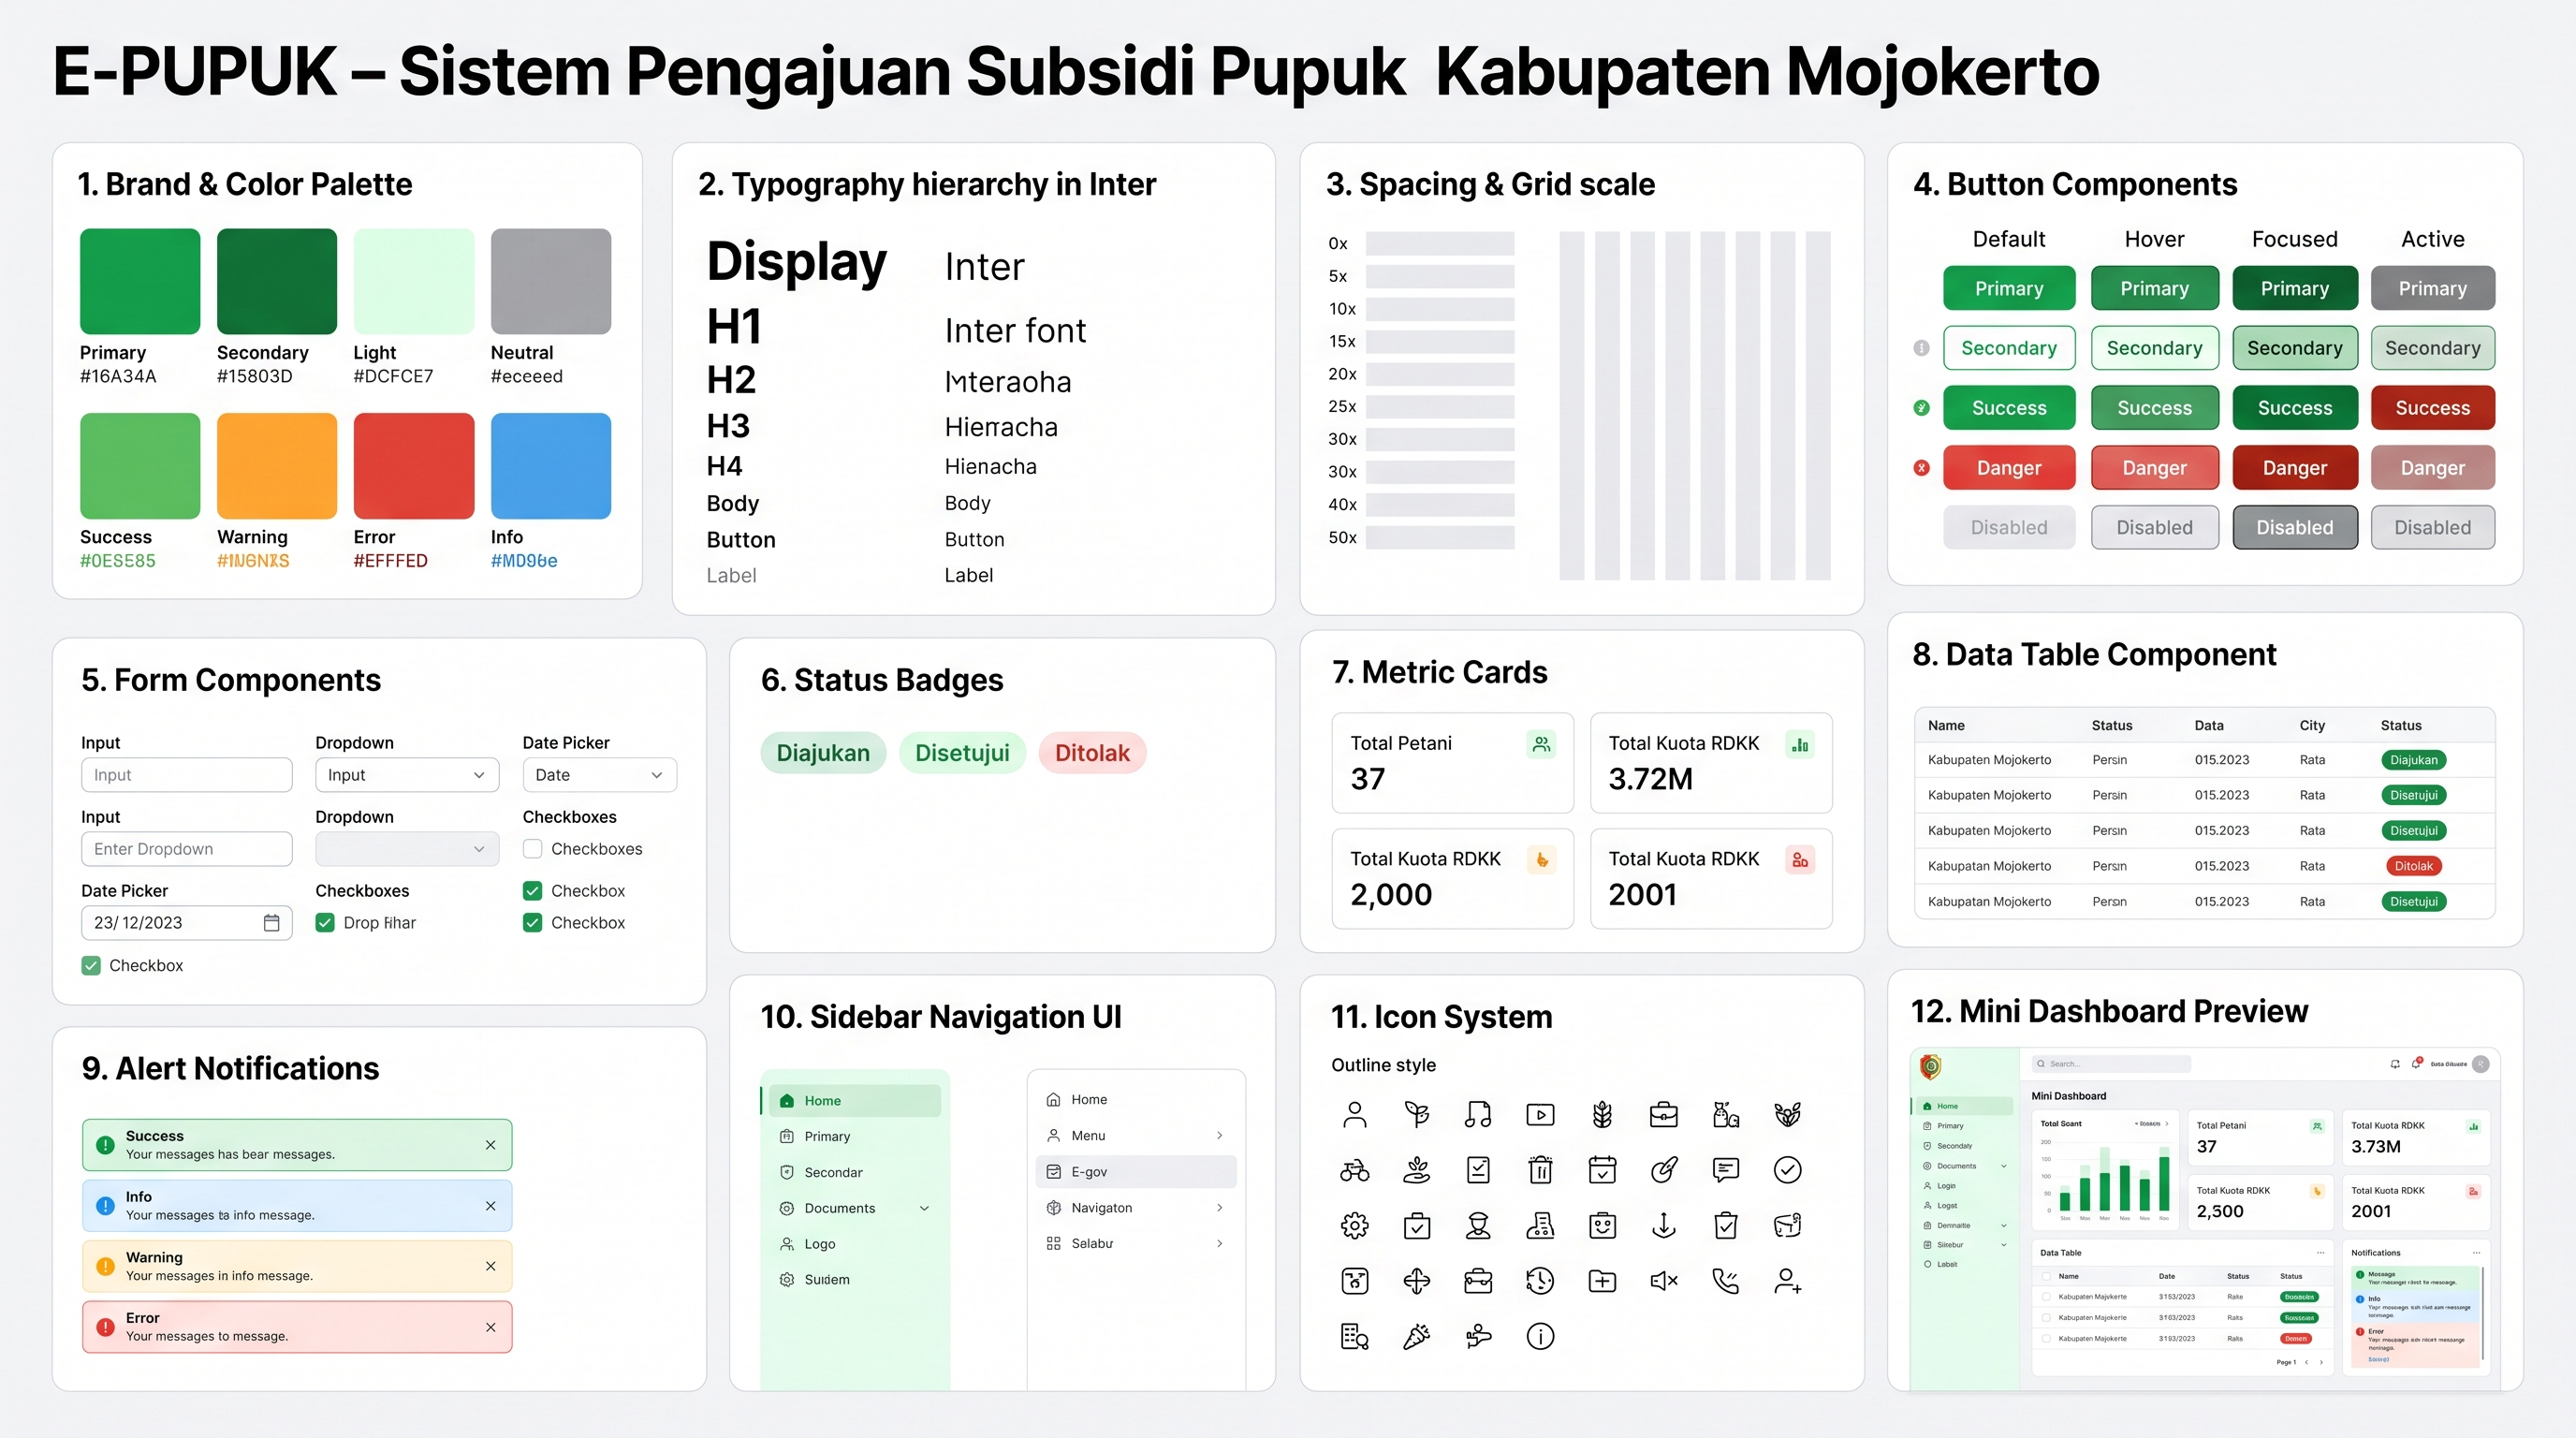
\includegraphics[width=0.9\textwidth]{design system.png}
    \caption{Design System E-Pupuk}
    \label{fig:design_system}
\end{figure}

\clearpage

% ==================== BAB IV ====================
\section{Arsitektur sistem}
\label{sec:arsitektur_sistem}

Arsitektur sistem E-Pupuk mengintegrasikan komponen frontend (React Web App), backend REST API (Python FastAPI), serta basis data terpusat (MySQL). Data terbuka pemerintah dimanfaatkan melalui modul data-seeding untuk memberikan informasi baseline kuota RDKK dan luas lahan.

\begin{figure}[htbp]
    \centering
    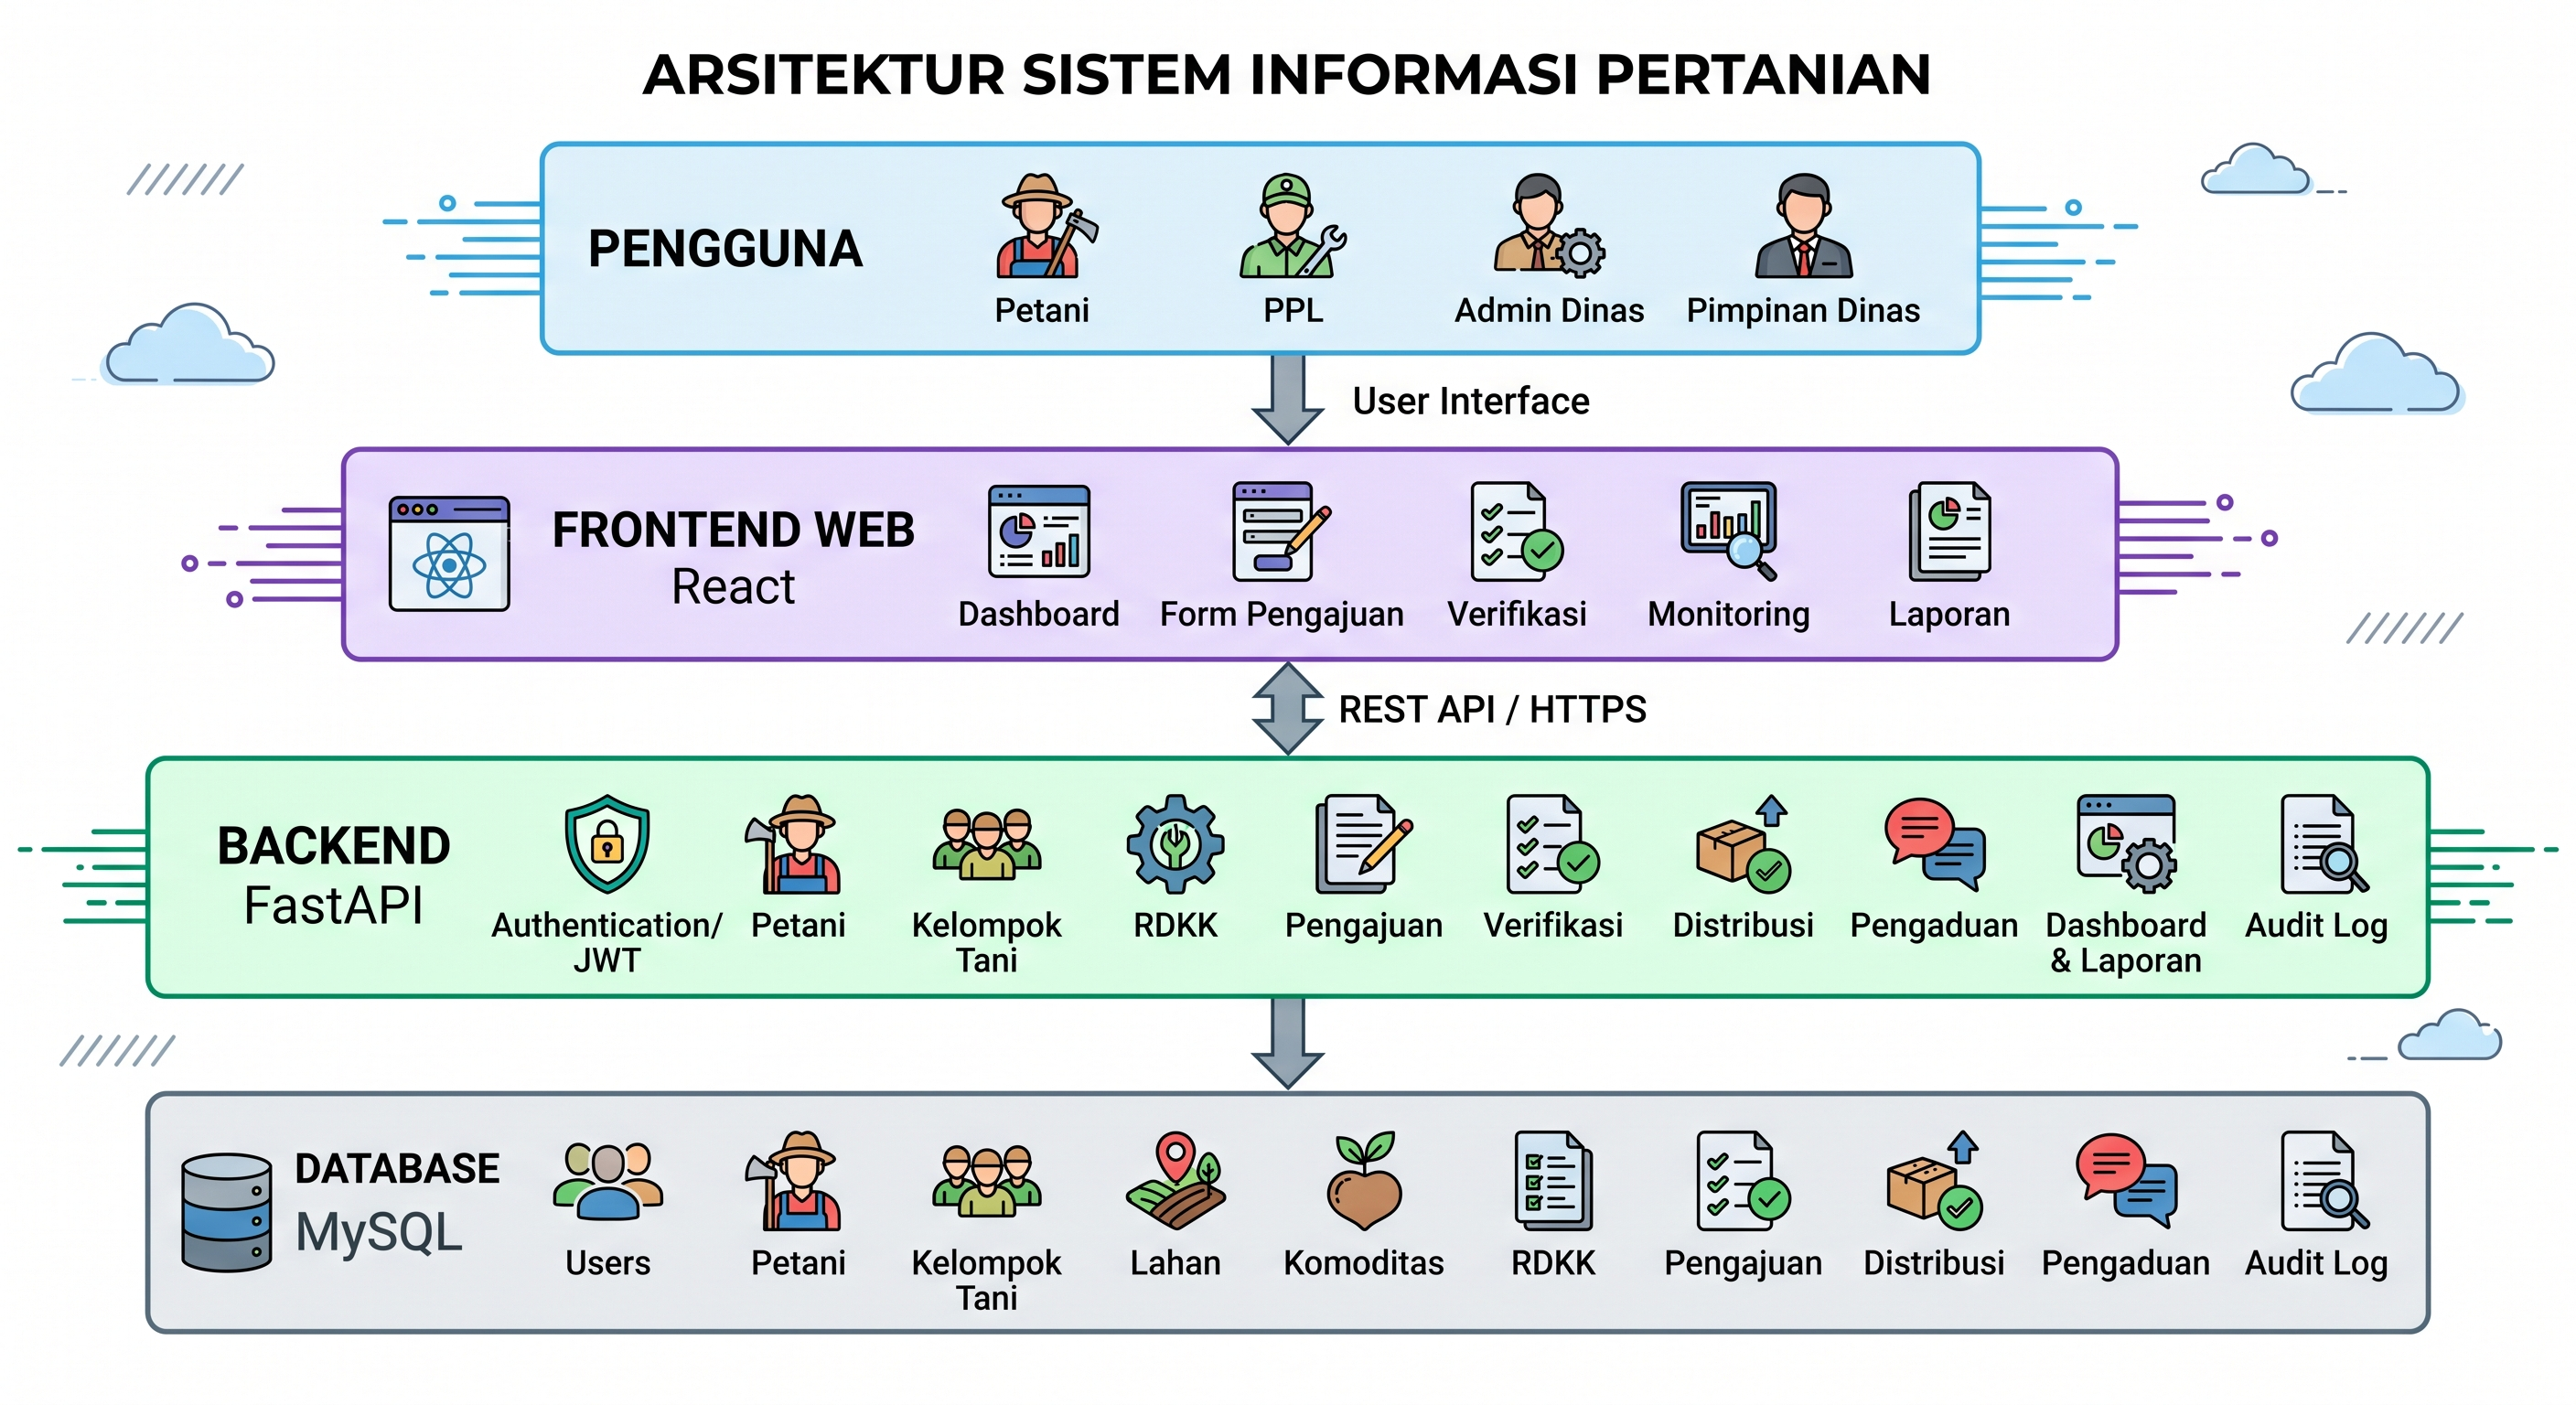
\includegraphics[width=0.9\textwidth]{arsitektur sistem.png}
    \caption{Arsitektur Sistem E-Pupuk}
    \label{fig:architecture_system}
\end{figure}

\clearpage

% ==================== BAB V ====================
\section{Mockup UI}
\label{sec:mockup_ui}

Bab ini menyajikan 5 rancangan antarmuka (\textit{Mockup UI}) utama sistem E-Pupuk dari folder \textit{Frontend} yang mencakup alur proses pengguna dari halaman utama, pengajuan petani, verifikasi PPL, hingga monitoring eksekutif Dinas Pertanian.

\begin{figure}[htbp]
    \centering
    \includegraphics[width=0.85\textwidth,height=0.65\textheight,keepaspectratio]{{Frontend/Beranda E-Pupuk Mojokerto - Agri-Gov Blue}.png}
    \caption{Mockup UI -- Halaman Utama / Beranda E-Pupuk Kabupaten Mojokerto}
    \label{fig:mockup_beranda}
\end{figure}

\clearpage

\begin{figure}[htbp]
    \centering
    \includegraphics[width=0.85\textwidth,height=0.65\textheight,keepaspectratio]{{Frontend/Dashboard Petani - Agri-Gov Blue}.png}
    \caption{Mockup UI -- Dashboard Petani (Informasi Kuota RDKK dan Status Lahan)}
    \label{fig:mockup_dashboard_petani}
\end{figure}

\clearpage

\begin{figure}[htbp]
    \centering
    \includegraphics[width=0.85\textwidth,height=0.65\textheight,keepaspectratio]{{Frontend/Ajukan Kebutuhan Pupuk - Agri-Gov Blue}.png}
    \caption{Mockup UI -- Form Pengajuan Kebutuhan Pupuk Subsidi oleh Petani}
    \label{fig:mockup_pengajuan}
\end{figure}

\clearpage

\begin{figure}[htbp]
    \centering
    \includegraphics[width=0.85\textwidth,height=0.65\textheight,keepaspectratio]{{Frontend/Detail Verifikasi Pengajuan - PPL Mojokerto}.png}
    \caption{Mockup UI -- Halaman Verifikasi Pengajuan Pupuk oleh Petugas Penyuluh Lapangan (PPL)}
    \label{fig:mockup_verifikasi_ppl}
\end{figure}

\clearpage

\begin{figure}[htbp]
    \centering
    \includegraphics[width=0.85\textwidth,height=0.65\textheight,keepaspectratio]{{Frontend/Dashboard Monitoring Eksekutif - E-Pupuk Mojokerto}.png}
    \caption{Mockup UI -- Dashboard Monitoring Eksekutif Dinas Pertanian}
    \label{fig:mockup_dashboard_eksekutif}
\end{figure}

\end{document}
\end{lstlisting}

\clearpage

% ==================== BAB III ====================
\section{Design System}
\label{sec:design_system}

Design system E-Pupuk merancang visual konsisten, komponen antarmuka modular, skema warna yang harmonis, dan elemen navigasi intuitif untuk pengguna dari berbagai peran (Petani, PPL, Admin, dan Pimpinan Dinas).

\begin{figure}[htbp]
    \centering
    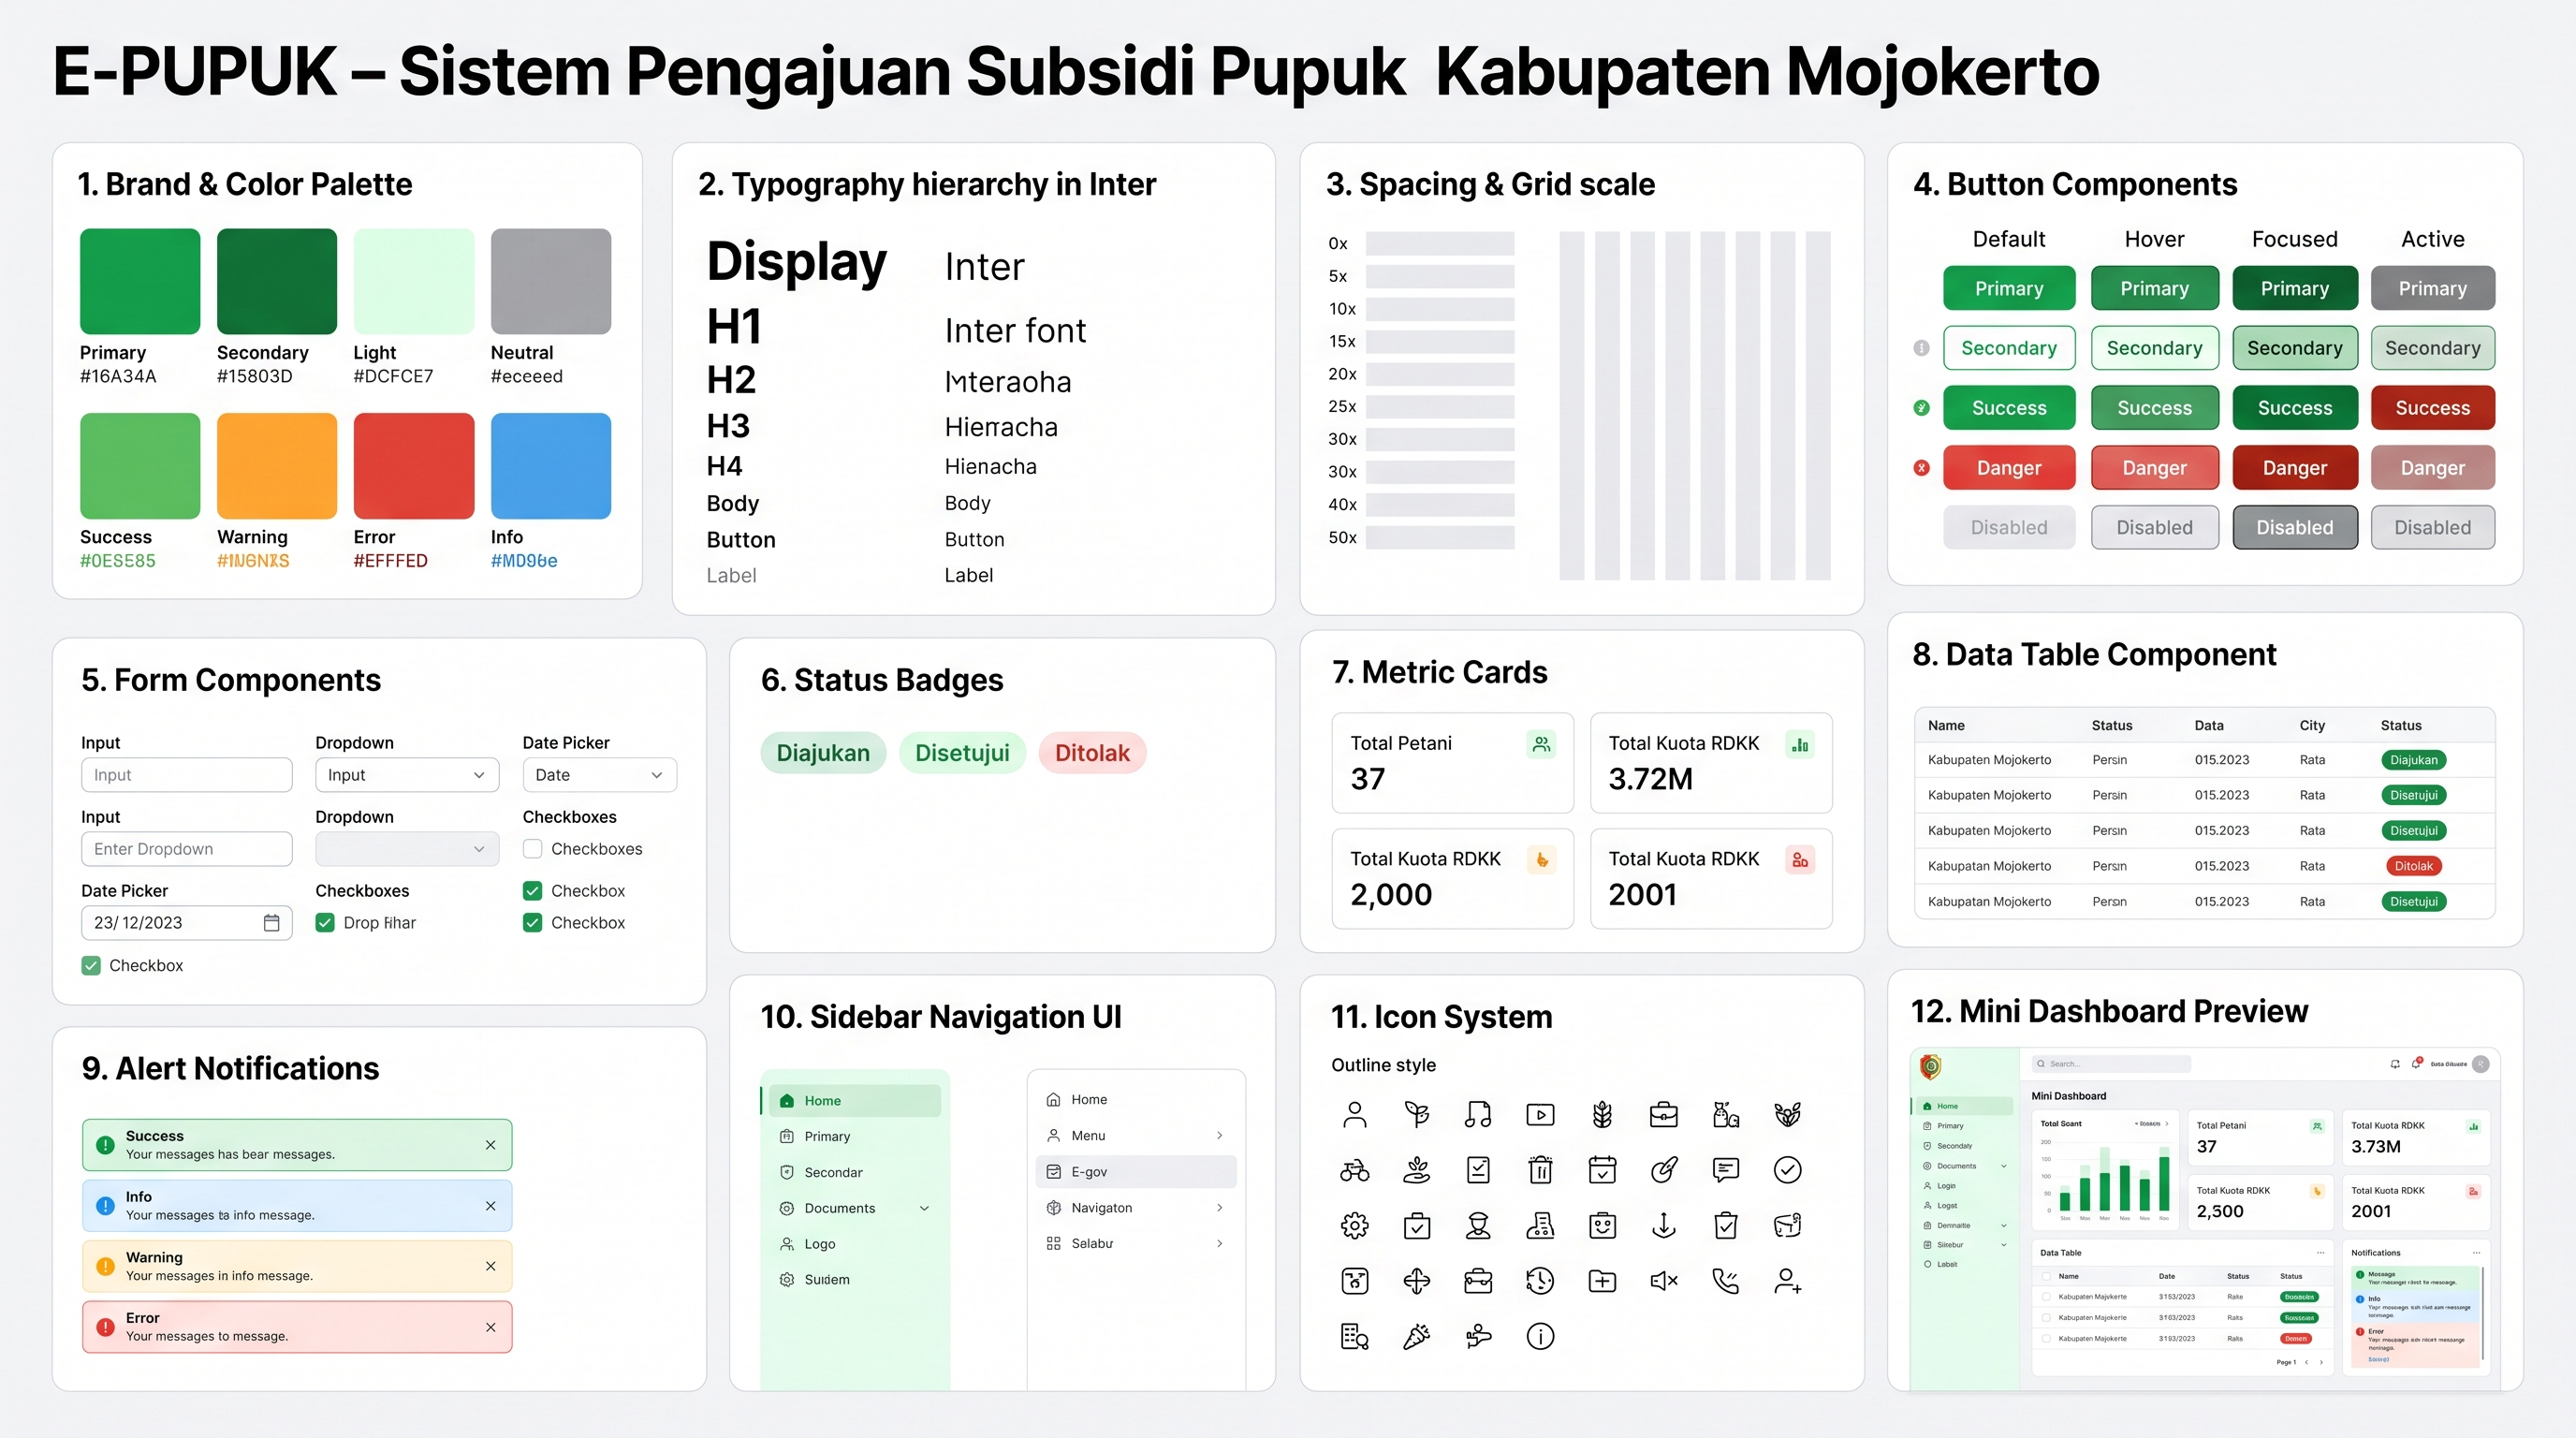
\includegraphics[width=0.9\textwidth]{design system.png}
    \caption{Design System E-Pupuk}
    \label{fig:design_system}
\end{figure}

\clearpage

% ==================== BAB IV ====================
\section{Arsitektur sistem}
\label{sec:arsitektur_sistem}

Arsitektur sistem E-Pupuk mengintegrasikan komponen frontend (React Web App), backend REST API (Python FastAPI), serta basis data terpusat (MySQL). Data terbuka pemerintah dimanfaatkan melalui modul data-seeding untuk memberikan informasi baseline kuota RDKK dan luas lahan.

\begin{figure}[htbp]
    \centering
    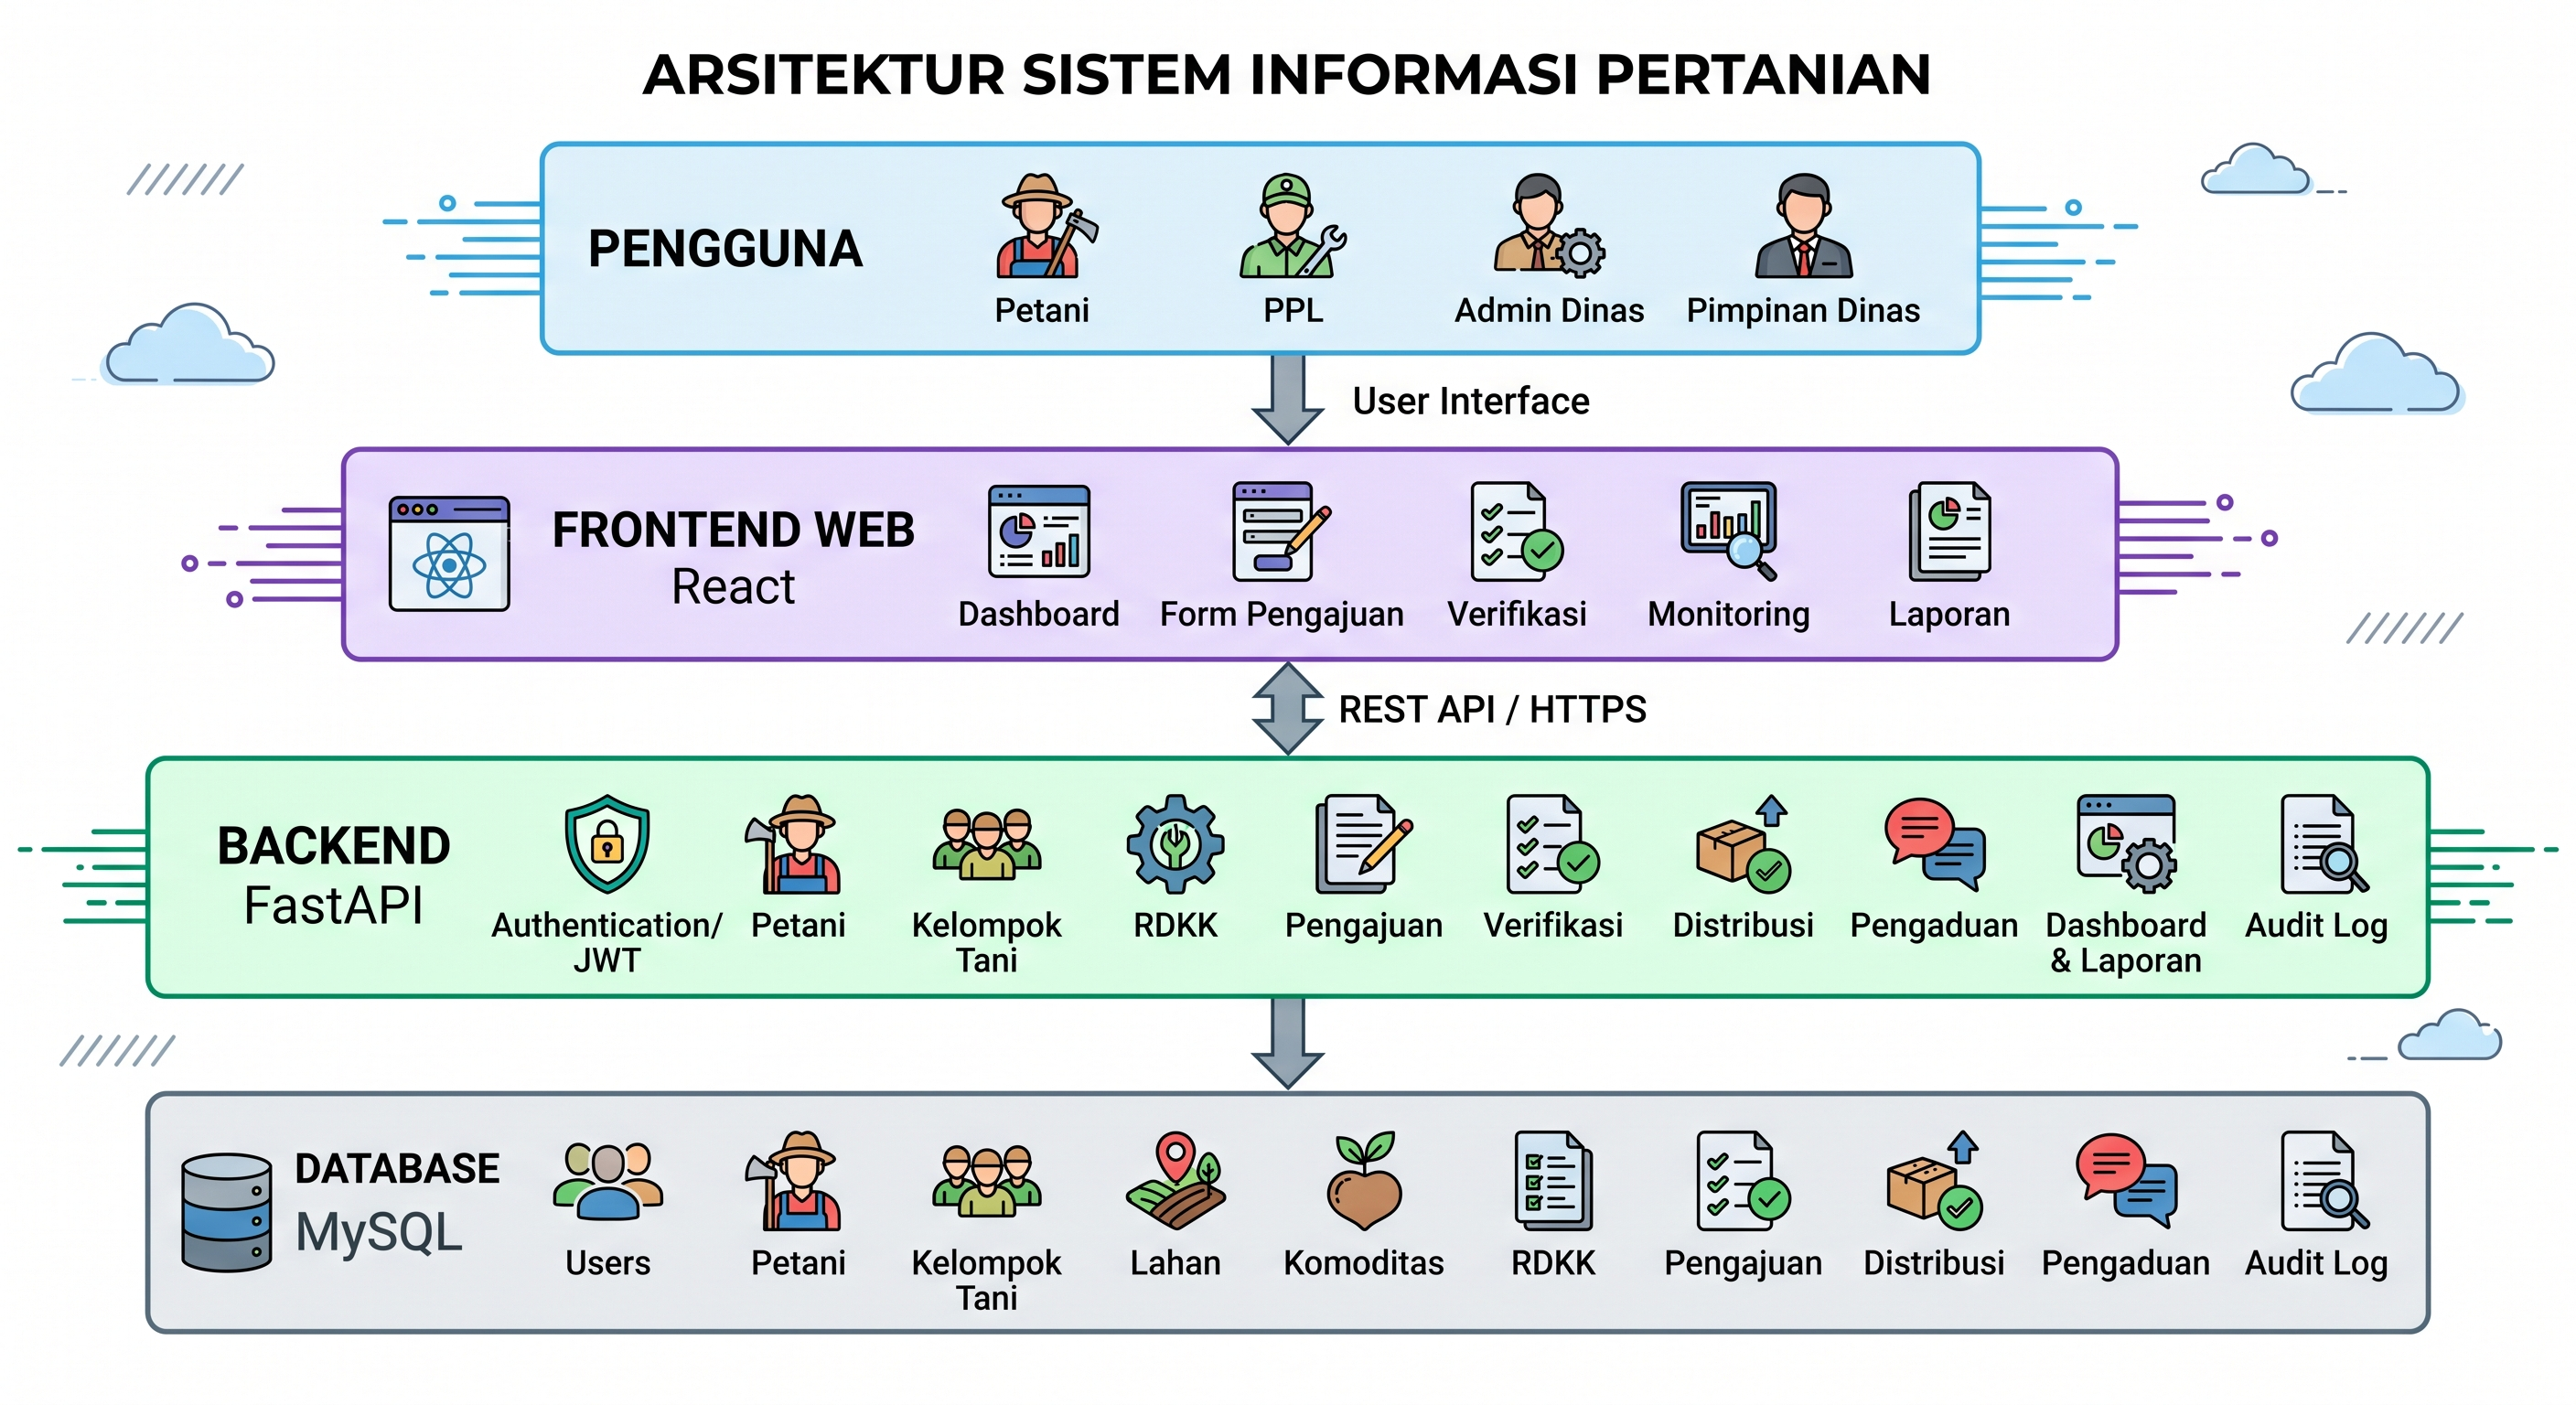
\includegraphics[width=0.9\textwidth]{arsitektur sistem.png}
    \caption{Arsitektur Sistem E-Pupuk}
    \label{fig:architecture_system}
\end{figure}

\clearpage

% ==================== BAB V ====================
\section{Mockup UI}
\label{sec:mockup_ui}

Bab ini menyajikan 5 rancangan antarmuka (\textit{Mockup UI}) utama sistem E-Pupuk dari folder \textit{Frontend} yang mencakup alur proses pengguna dari halaman utama, pengajuan petani, verifikasi PPL, hingga monitoring eksekutif Dinas Pertanian.

\begin{figure}[htbp]
    \centering
    \includegraphics[width=0.85\textwidth,height=0.65\textheight,keepaspectratio]{{Frontend/Beranda E-Pupuk Mojokerto - Agri-Gov Blue}.png}
    \caption{Mockup UI -- Halaman Utama / Beranda E-Pupuk Kabupaten Mojokerto}
    \label{fig:mockup_beranda}
\end{figure}

\clearpage

\begin{figure}[htbp]
    \centering
    \includegraphics[width=0.85\textwidth,height=0.65\textheight,keepaspectratio]{{Frontend/Dashboard Petani - Agri-Gov Blue}.png}
    \caption{Mockup UI -- Dashboard Petani (Informasi Kuota RDKK dan Status Lahan)}
    \label{fig:mockup_dashboard_petani}
\end{figure}

\clearpage

\begin{figure}[htbp]
    \centering
    \includegraphics[width=0.85\textwidth,height=0.65\textheight,keepaspectratio]{{Frontend/Ajukan Kebutuhan Pupuk - Agri-Gov Blue}.png}
    \caption{Mockup UI -- Form Pengajuan Kebutuhan Pupuk Subsidi oleh Petani}
    \label{fig:mockup_pengajuan}
\end{figure}

\clearpage

\begin{figure}[htbp]
    \centering
    \includegraphics[width=0.85\textwidth,height=0.65\textheight,keepaspectratio]{{Frontend/Detail Verifikasi Pengajuan - PPL Mojokerto}.png}
    \caption{Mockup UI -- Halaman Verifikasi Pengajuan Pupuk oleh Petugas Penyuluh Lapangan (PPL)}
    \label{fig:mockup_verifikasi_ppl}
\end{figure}

\clearpage

\begin{figure}[htbp]
    \centering
    \includegraphics[width=0.85\textwidth,height=0.65\textheight,keepaspectratio]{{Frontend/Dashboard Monitoring Eksekutif - E-Pupuk Mojokerto}.png}
    \caption{Mockup UI -- Dashboard Monitoring Eksekutif Dinas Pertanian}
    \label{fig:mockup_dashboard_eksekutif}
\end{figure}

\end{document}
